\justifying
\noindent

\section{Sensor Technology}
This section of the paper will focus on sensor technology, Specifically in LCD Display and Infrared Imaging (Thermography). This section will include brief introduction, system mechanism, and real-life application for each type of categories

\subsection{Liquid-Crystal Display (LCD)}
\noindent Liquid-Crystal Display has become one of the major usage in any display application due to its low power consumption than its competitor such as LED or Cathode Ray Tube (CRT). The application of LCD range from basic 8-bit numbering display to high-pixel colour display such as television. liquid crystal refers to the state of a matter that has two distinct melting point which combines both two states of matter, solid and liquid \cite{AnonymousLCDApplications}\cite{Gurski2005DisplayOverview}. The application of an electric or magnetic field allows the manipulation of molecules orientation to a predicted manner which become the basis of LCD, moreover, the principle of LCD is to block the light from the backlight emitted \cite{Gurski2005DisplayOverview}.\\

\begin{figure}[!ht]
\begin{center}
%    
  \begin{subfigure}[b]{0.4\textwidth}
    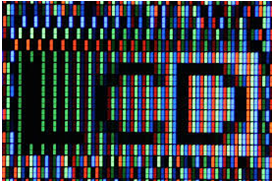
\includegraphics[height=4cm]{Figures/LCD_general.PNG}
  \end{subfigure}
  %
  \begin{subfigure}[b]{0.35\textwidth}
    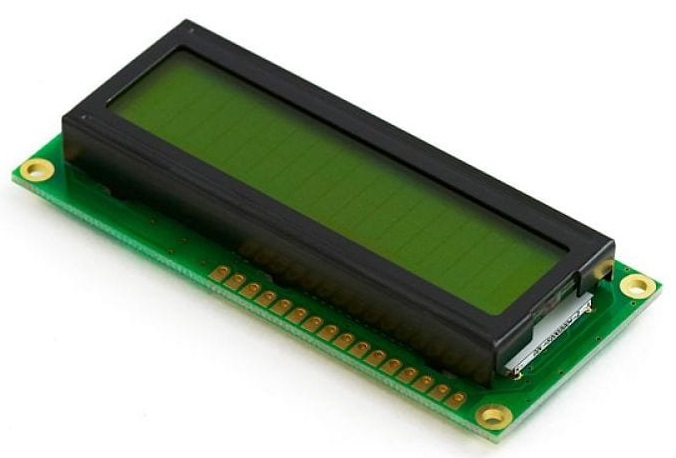
\includegraphics[height=4cm]{Figures/LCD_BASIC.jpg}
  \end{subfigure}
%  
  \caption{An LCD Representation \cite{Gurski2005DisplayOverview} (left) and basic character LCD \cite{AnonymousBasicSystems} (right).}
    \label{fig:basic lcd}
\end{center}
\end{figure}


\noindent A typical construction of typical LCD shown in figure \ref{fig:LCD structure} below. The first structure is the backlight source followed with bottom polarisers which perpendicular to each other in purpose of molecules alignment when current is applied. Thin-film-transistor (TFT) and glass substrate which are one of liquid crystal, and colour filter and black matrix are placed in between the polarisers \cite{AnonymousLCDApplications}. \\ 

\noindent The LCD works by untwisting the molecules by applying current to the liquid-crystal. This allows the angle of light passes through the molecules of the bottom polarised filter and changed the angle of top polarising filter. All this mechanism allows the light to pass the small amount of light through the particular area of the LCD, therefore creating a more dark region compared to others.

\begin{figure}[!ht]
    \centering
    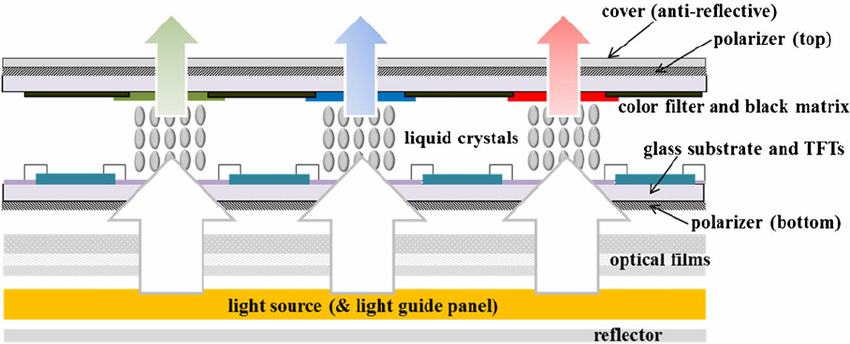
\includegraphics[scale=0.4]{Figures/LCD_Typical structure.png}
    \caption{A Typical structure of an LCD \cite{Park2013EfficiencyPrograms}}
    \label{fig:LCD structure}
\end{figure}

\subsubsection{General Navigation Panel}
The most common use of an LCD panel is to aid and support the navigation by applying a simple display to a coordinate or frequency. In the modern technologies, LCD has developed into a  high-definition (HD) colour display which allows advance applications (camera view, GPS, etc)  rather than showing a basic character. In modern aircraft such as Airbus A350 and Boeing 787 use large multi-functional display units \cite{AnonymousTouchAirbus} and this system are usually based on full colour matrix LCD. Figure \ref{fig:avionics 5inc} below shows 5 inch LCD avionics display in an aircraft cockpit and general avionics LCD composition.

\begin{figure}[!ht]
\begin{center}
%    
  \begin{subfigure}[b]{0.4\textwidth}
    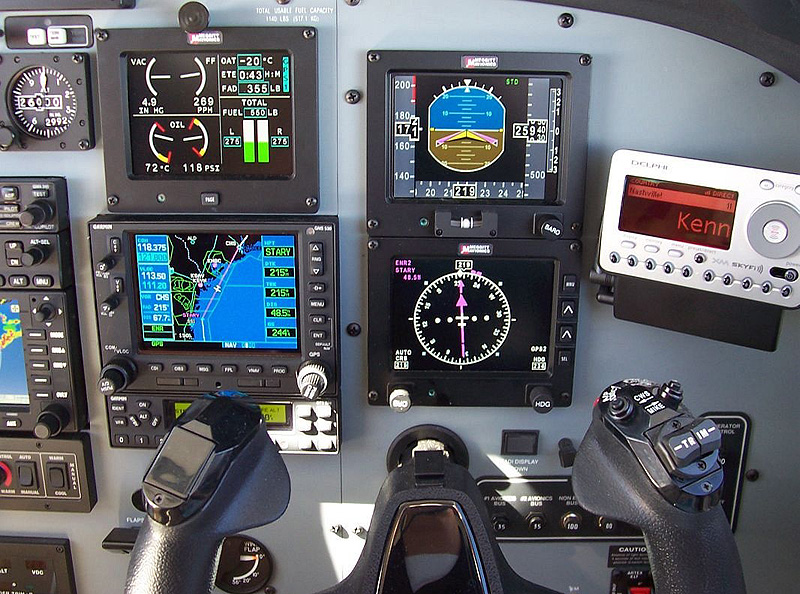
\includegraphics[height=5cm]{Figures/LCD_Avionics_5inch.jpg}
  \end{subfigure}
  %
  \begin{subfigure}[b]{0.35\textwidth}
    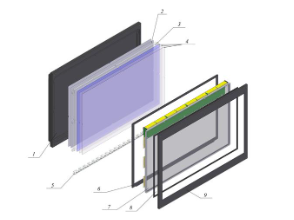
\includegraphics[height=5cm]{Figures/LCD_avionics_composition.PNG}
  \end{subfigure}
%  
  \caption{LCD application of avionics display on a Piper aircraft cockpit \cite{Anonymous5LCD} (left) and Avionics LCD Composition diagram \cite{Alimova2020MethodsApplications} (right).}
    \label{fig:avionics 5inc}
\end{center}
\end{figure}


\subsection{Infrared Imaging (Thermography)}
\subsubsection{Forward Looking Infrared (FLIR) - Surveillance}
\subsubsection{Aviation heat thingy}